%%%%%%%%%%%%%%%%%%%%%%%%%%%%%%%%%%%%%%%%%%%%%%%%%%%
%
%  New template code for TAMU Theses and Dissertations starting Fall 2016.
%
%
%  Author: Sean Zachary Roberson 
%	 Version 3.16.09
%  Last updated 9/12/2016
%
%%%%%%%%%%%%%%%%%%%%%%%%%%%%%%%%%%%%%%%%%%%%%%%%%%%

%%%%%%%%%%%%%%%%%%%%%%%%%%%%%%%%%%%%%%%%%%%%%%%%%%%%%%%%%%%%%%%%%%%%%%
%%                           APPENDIX A 
%%%%%%%%%%%%%%%%%%%%%%%%%%%%%%%%%%%%%%%%%%%%%%%%%%%%%%%%%%%%%%%%%%%%%
\phantomsection
\chapter{\uppercase {Analysis of Anomalous GFEM Seismograms}}
In this appendix I analyze the anomalous results obtained in two of the 100 receiver arrays for the scattering model presented in section 3. These irregular outputs are evident in Figures \ref{fig:3.35} and \ref{fig:3.36} which show the maximum correlation lag and two types of error for GFEM simulation cases obtained with 5 plane wave directions. In these figures, the results corresponding to the receivers placed at 467.2 and 474.2 m  are outliers that  strongly deviate from the average trend. 

Figure \ref{fig:a.1} shows traces for the reference solution and for the GFEM solution presenting the aforementioned issues in the red colored red trace. Notice that the traces for the FEM solution smoothly shift in time from receiver to receiver. However, for the GFEM solution, the two traces in red present abrupt changes.
Figure \ref{fig:a.2} show the maximum cross correlation lag and errors for the receiver array for this GFEM solution, together with the highlighted cells for which the corresponding receivers present spikes in the results.
Figures \ref{fig:a.2} and \ref{fig:a.4} show similar outputs as in Figure \ref{fig:a.2}. However for this cases the receiver spacing has been increased by 0.1 m and 0.2 m correspondingly to obtain the GFEM solutions. Notice that in Figure \ref{fig:a.3}(a) there is only one spike present and that in \ref{fig:a.3}(b) there is not a receiver located to the left of the  highlighted grid,  and that the highlighted grid is the same as one of the shaded ones in the previous Figure. In Figure \ref{fig:a.4}, two spikes are visible again corresponding to the same grids as in Figure \ref{fig:a.2}.
Although these observations do not provide with the underlying cause for these anomalies, it suggest that for the mesh used for these GFEM cases, this errors are associated with receivers located at the highlighted grids in Figures \ref{fig:a.2} and \ref{fig:a.3}. However, further investigation is needed to find the source of these systematic irregularity.


 \begin{figure}[h!]
 		\centering
		\begin{subfigure}{8cm}
				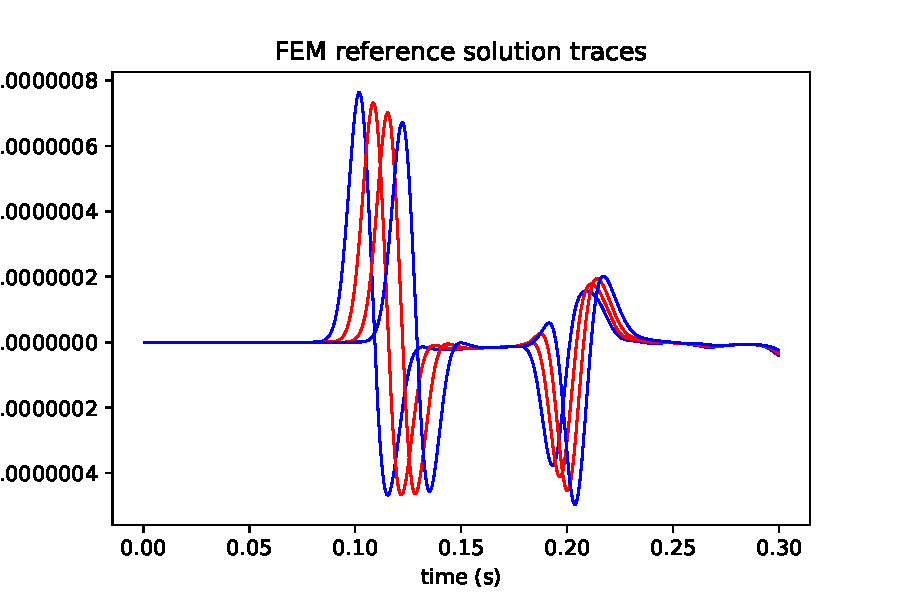
\includegraphics[width=8cm, height=6cm]{Thesis_Edith/figures/scattering/appendix/fem_scat_traces.pdf}
			     \caption{}
				%\label{fig:trace1}
		\end{subfigure}
        \hspace{0.25cm}
		\begin{subfigure}{8cm}
				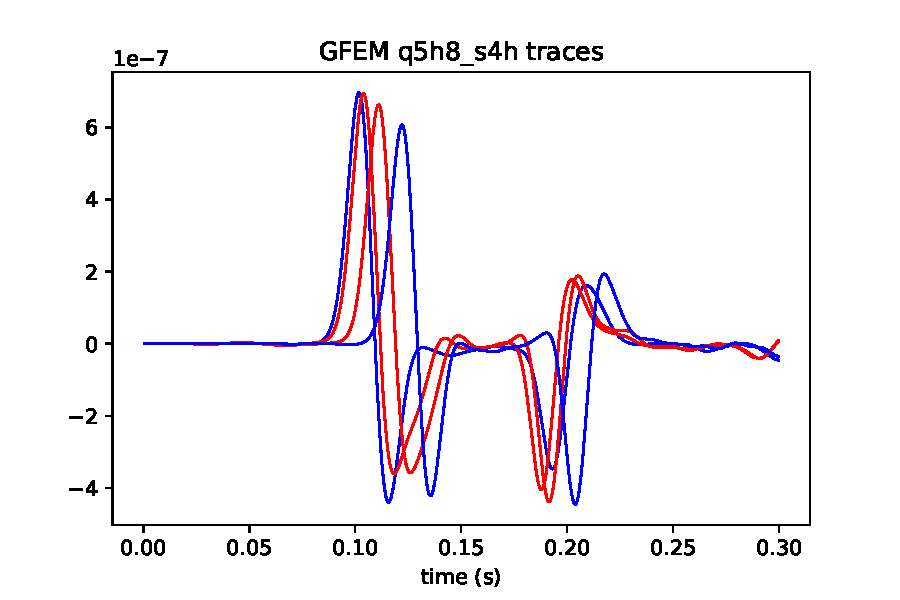
\includegraphics[width=8cm, height=6cm]{Thesis_Edith/figures/scattering/appendix/gfem_scat_traces.pdf}
			   \caption{}
				%\label{fig:trace3}
		\end{subfigure}
 
	\caption{Scattering model: (a) Traces for the FEM reference solution, red colored traces belong to those that present an anomaly in the GFEM cases in question. (b) Traces for a GFEM solution showing in red those that deviates from the average trend.}  
	\label{fig:a.1}
\end{figure}

%spacing 7 m
\begin{figure}[h!]
 		\centering
		\begin{subfigure}{8cm}
				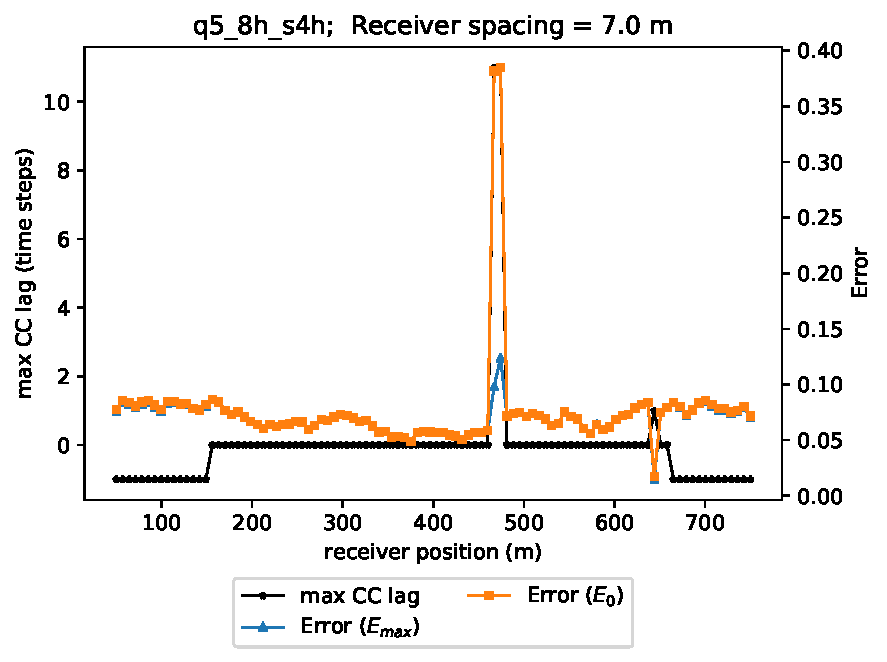
\includegraphics[width=8cm, height=6cm]{Thesis_Edith/figures/scattering/appendix/spike7.pdf}
			     \caption{}
				%\label{fig:trace1}
		\end{subfigure}
        \hspace{0.25cm}
		\begin{subfigure}{8cm}
				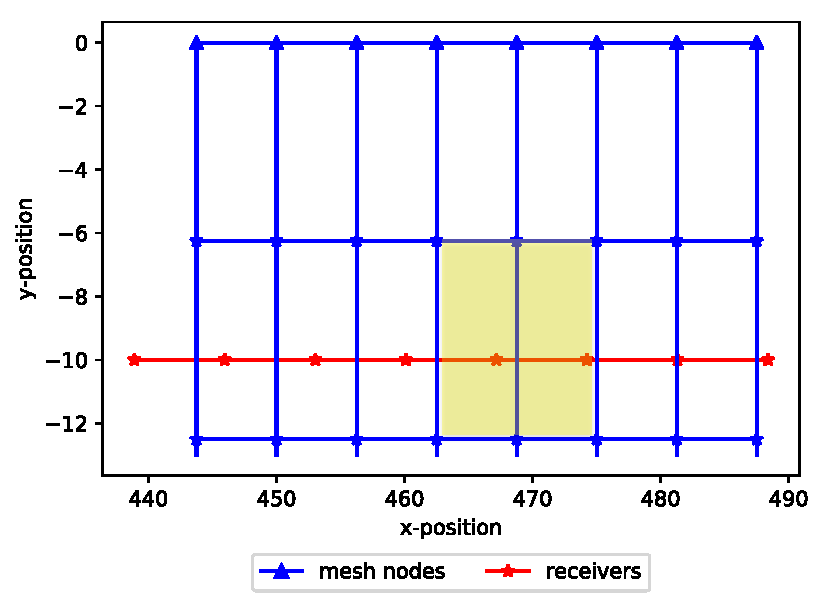
\includegraphics[width=8cm, height=6cm]{Thesis_Edith/figures/scattering/appendix/receiver-spacing1_v2.pdf}
			   \caption{}
				%\label{fig:trace3}
		\end{subfigure}
 
	\caption{Scattering model: (a) Maximum cross correlation lag and errors for the GFEM case in Figure \ref{fig:a.1}(b). (b) Mesh grid and receiver location with highlighted grids corresponding to the receiver positions where the spikes occur.}  
	\label{fig:a.2}
\end{figure}

%spacing 7.1 m
\begin{figure}[h!]
 		\centering
		\begin{subfigure}{8cm}
				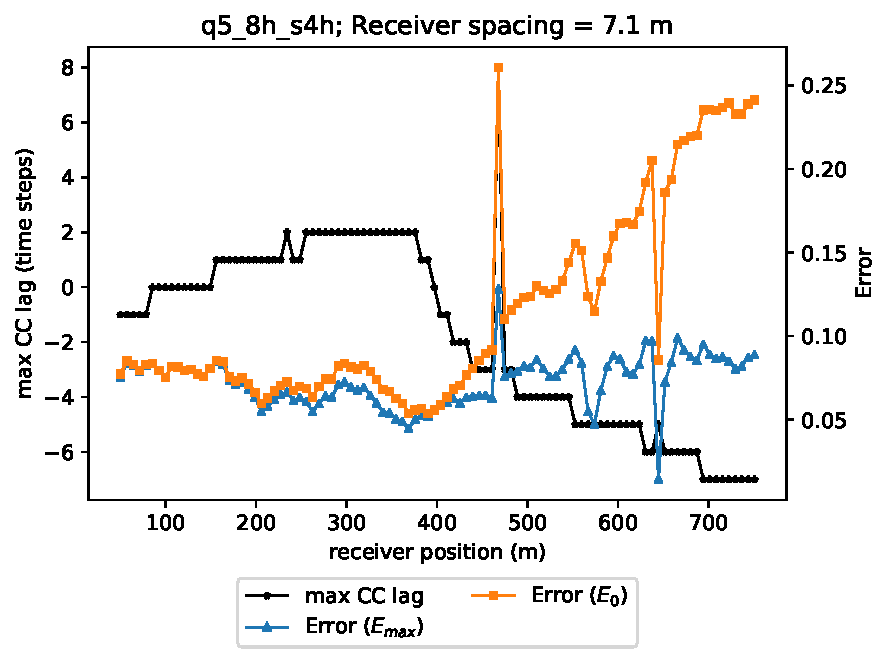
\includegraphics[width=8cm, height=6cm]{Thesis_Edith/figures/scattering/appendix/spike7_1.pdf}
			     \caption{}
				%\label{fig:trace1}
		\end{subfigure}
        \hspace{0.25cm}
		\begin{subfigure}{8cm}
				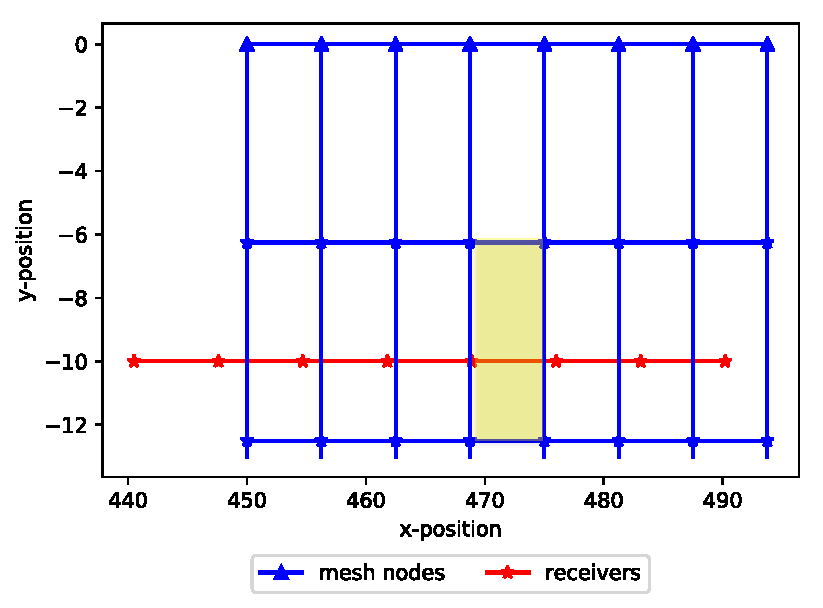
\includegraphics[width=8cm, height=6cm]{Thesis_Edith/figures/scattering/appendix/receiver-spacing3_v2.pdf}
			   \caption{}
				%\label{fig:trace3}
		\end{subfigure}
 
	\caption{Scattering model: Figures obtained when shifting the receivers 0.1 m to the right for the GFEM solution. (a) Maximum cross correlation lag and error for the GFEM solution. (b) Mesh grid and receiver location with highlighted grids corresponding to the receiver position where the spikes occur}  
	\label{fig:a.3}
\end{figure}

%spacing 7.2 m
\begin{figure}[h!]
 		\centering
		\begin{subfigure}{8cm}
				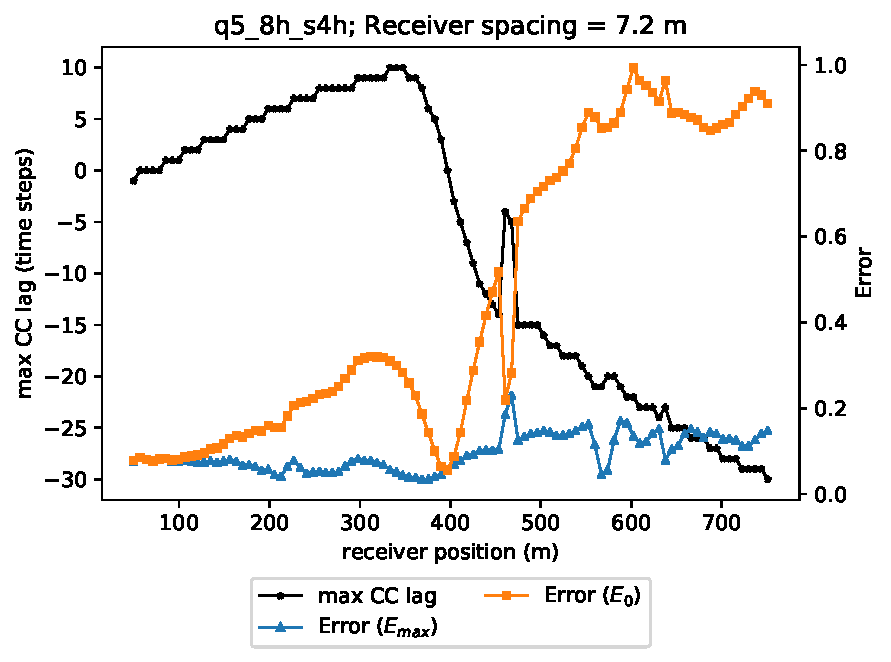
\includegraphics[width=8cm, height=6cm]{Thesis_Edith/figures/scattering/appendix/spike7_2.pdf}
			     \caption{}
				%\label{fig:trace1}
		\end{subfigure}
        \hspace{0.25cm}
		\begin{subfigure}{8cm}
				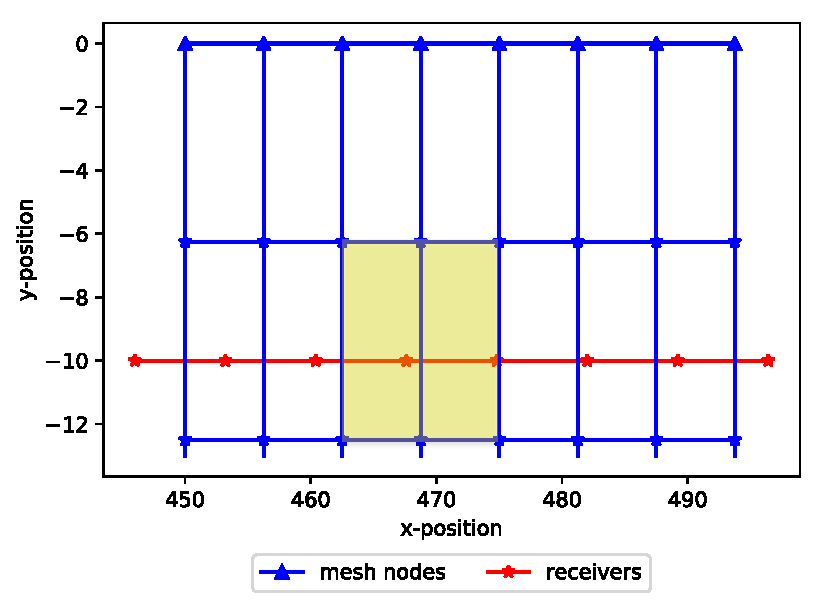
\includegraphics[width=8cm, height=6cm]{Thesis_Edith/figures/scattering/appendix/receiver-spacing4_v2.pdf}
			   \caption{}
				%\label{fig:trace3}
		\end{subfigure}
 
	\caption{Scattering model: Figures obtained when shifting the receivers 0.2 m to the right for the GFEM solution. (a) Maximum cross correlation lag and error for the GFEM solution. (b) Mesh grid and receiver location with highlighted grids corresponding to the receiver positions where the spikes occurs. }  
	\label{fig:a.4}
\end{figure}


%  \begin{figure}[h!]
% 	\centering
% 	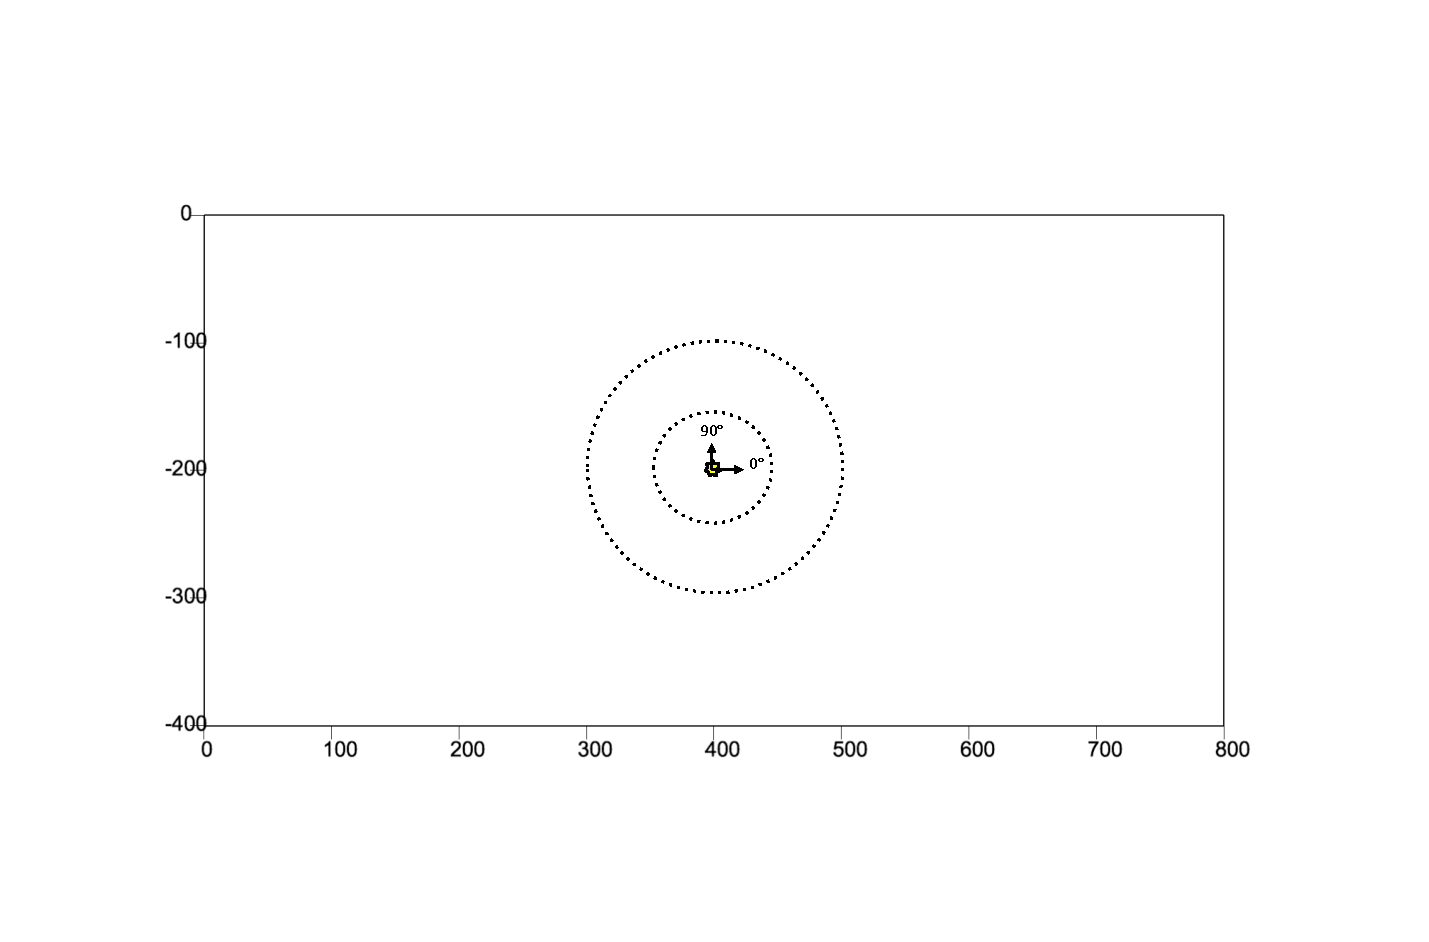
\includegraphics[width=12cm, height=6.5cm]{Thesis_Edith/figures/homo/h_source.pdf}
% 	\caption{Homogeneous model with a seismic source in the center (yellow star) and two sets of receiver arrays (dotted circles) at 50 m and at 100 m from the center of the source.}
% 	\label{fig:3.1}
% \end{figure}